\chapter{绪论}
\section{自旋电子学概述}
自旋电子学是一种新型电子学技术,与传统电子学依靠电子的电荷自由度不同,它利用电子的自旋自由度来传输、存储和处理信息。
从上世纪80年代观察到的磁电阻现象起,自旋电子学逐渐在磁性存储器、传感器、计算机和通信设备等领域展现出了广泛的应用前景。
由于它的应用涉及到电子自旋的操纵、传输和检测,而自旋与磁性密切相关,因此磁性材料在自旋电子学中具有重要的地位。
一些新型材料的发现也促进了自旋电子学的进一步发展,如半金属铁磁体(\ce{CrO2}和\,\ce{Fe3O4})、半金属反铁磁体、拓扑绝缘体和磁性半导体等。
此外,自旋电子学的研究还涉及到新的现象,如自旋霍尔效应和自旋轨道效应等,这些现象为自旋电子学的应用提供了新的机遇和挑战。\par
如今,自旋电子器件在数据存储的两个不同技术中发挥着重要作用。
一方面,自旋阀磁记录读取头大幅增加了磁性硬盘驱动器(HDD)的存储容量;另一方面,自旋电子学的发展为实现无运动机械部件的固态存储器提供了可能性。
其中,磁性随机存储器(MRAM)是一种非常有前景的存储技术,它将磁性元素的磁化方向代表数据信息进行存储。
2008年,Parkin等人\cite{parkin2008magnetic}提出了一种新型存储技术——基于磁畴壁的赛道存储器。
与现在的任何其他固态存储设备不同,这种存储器可以将编码在手性磁畴壁中的磁性数据沿着磁性纳米赛道移动,通过在单个赛道中存储许多磁畴壁(可能是 100
个或更多)就可以实现非常密集的存储。
这种潜在的固态非易失性存储器的存储容量可与磁盘驱动器相媲美,而且性能更好、能耗更低。\par
对于使用斯格明子作为赛道存储器数据位的兴趣是源于观察到单晶B20化合物\ \ce{MnSi}中的斯格明子可以用非常小的电流移动,这个电流密度比使用自旋轨道力矩
(SOT)驱动磁畴壁的临界电流密度还低几个数量级。%打一个空格使字间距不太紧密。
尽管非常低的电流密度会导致斯格明子运动非常缓慢,但对于一些赛道存储器的应用,例如替代垂直NAND闪存存储器,小电流密度是非常有利的,而且数据位的缓慢运动也是可以接受的。
基于斯格明子的赛道存储器给存储技术提供了一种新的选择,使赛道存储设备在更低的能耗和更高的读写速度之间取得平衡,这非常有吸引力并具有光明的应用前景。
\subsection{巨磁电阻(GMR)}
自旋极化电流从铁磁性(FM)材料注入到非磁性(NM)材料中是1975年的隧道磁电阻(TMR)、1988年的巨磁电阻(GMR)和1993年的Johnson晶体管演示所使用的最常用的产生自旋的方法,并由此开启了磁输运的研究\cite{julliere1975tunneling,baibich1988giant,binasch1989enhanced,johnson1991analysis}。
注入效率取决于铁磁材料的自旋极化和FM/NM界面处的自旋散射。
此外,消除铁磁材料的杂散场对于注入效率也非常重要。
磁输运的一个关键发现是由Fert\cite{baibich1988giant}和Grünberg\cite{binasch1989enhanced}发现的多层磁性金属材料中的巨磁电阻效应,他们因此发现获得了2007年的诺贝尔物理学奖。
巨磁电阻效应是指在一个金属层系统中,当外部磁场改变铁磁层的磁化时其电阻发生巨大变化\cite{ennen2016giant}。
两个铁磁层的磁矩平行排列通常比反平行排列时具有更低的电阻,如图\ref{图1.1}所示。
磁电阻比率($P_{MR}$)可以定义为:
\begin{equation}
    P_{MR} = \frac{\Delta R}{R} = \frac{R_{AP}-R_P}{R_P}
    \label{公式1-1}
\end{equation}
式中:$R_P$和$R_{AP}$分别表示两个铁磁层中磁化方向平行和反平行时的电阻。
1998年,IBM发现了称为自旋阀的低场GMR传感器。
相比于先前存在的基于各向异性磁电阻(AMR)的磁电阻传感器,这些传感器能够提供更大的信号变化,而且在硬盘驱动器中读取存储数据时具有更好的稳定性。
随后,在温度为\mySI{300}{K}下$\mathrm{[Co(0.8)/Cu(0.83)]_{60}}$(厚度单位为nm)结构中$P_{MR}$已经提高到65\% \cite{ikeda2008tunnel}。
通过将铁磁材料替换为半金属铁磁材料\ce{Co2FeGa_{0.5}Ge_{0.5}},室温下最大$P_{MR}$可达82\% \cite{parkin1991giant}。
\begin{figure}[h]
    \centering
    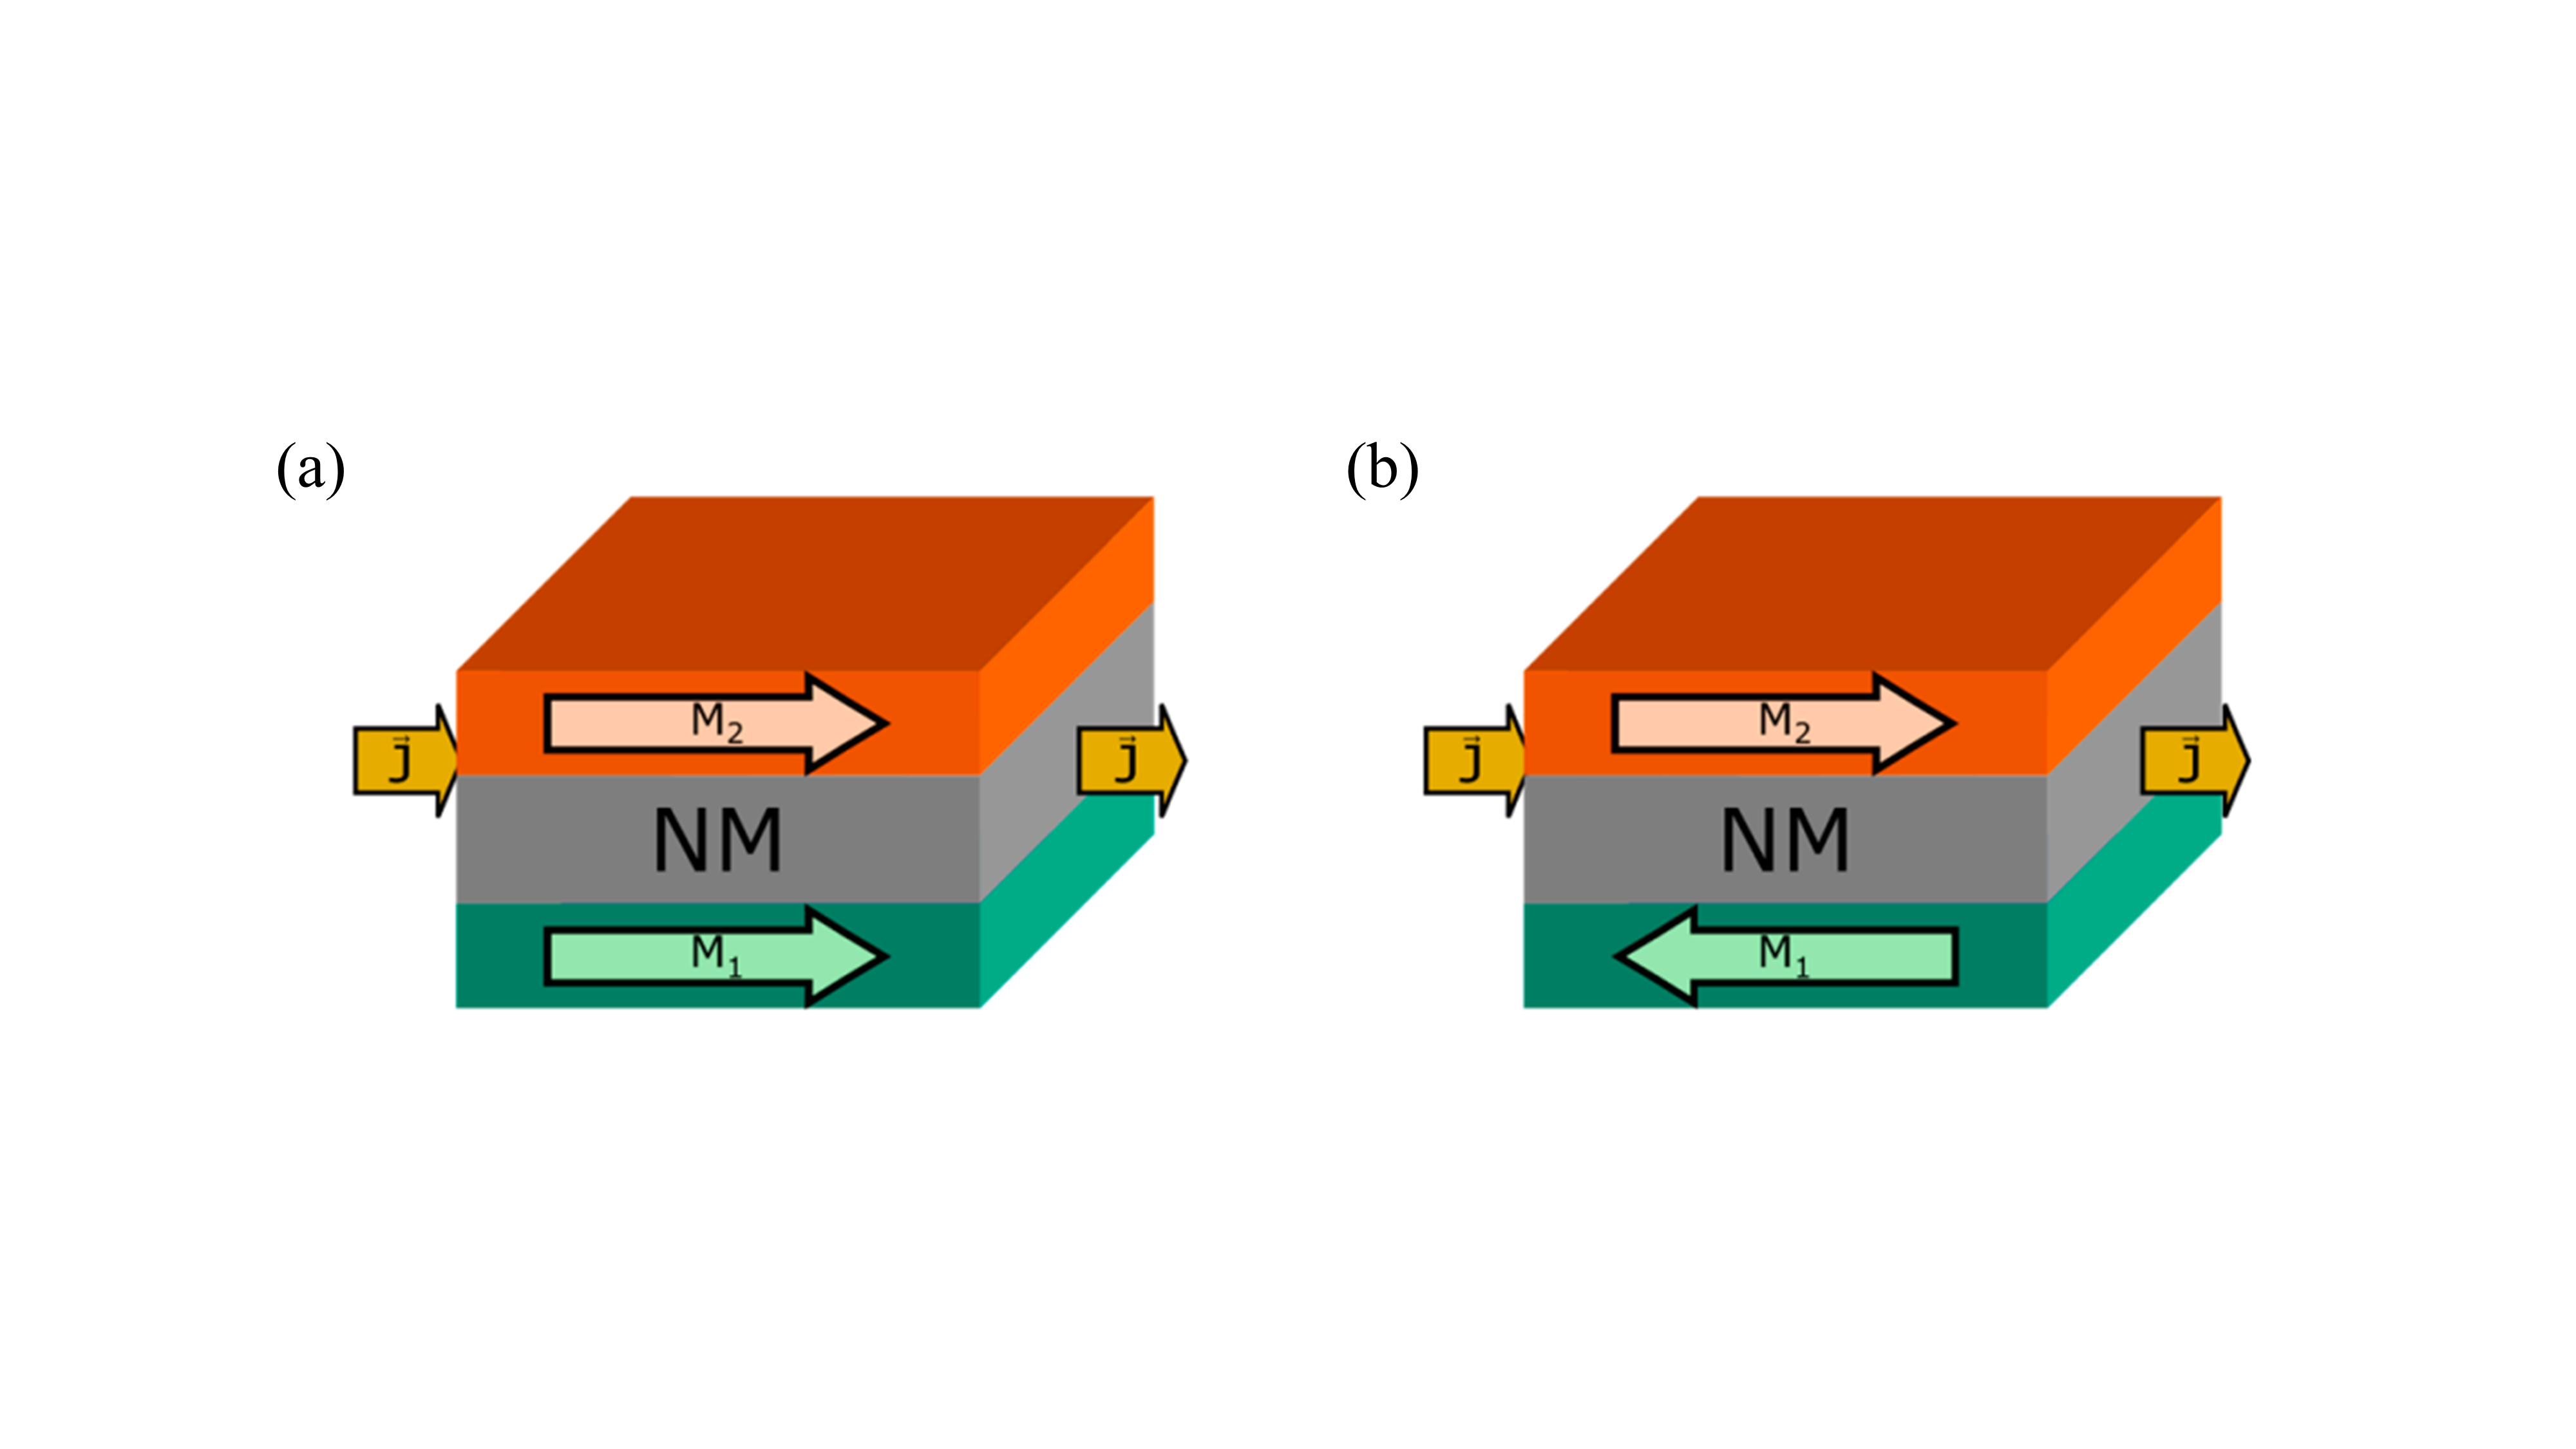
\includegraphics[width=\textwidth,trim=3cm 5.5cm 3cm 5.5cm,clip]{Figures/Chapter1/图片1.png}
    \bicaption{平面内电流(CIP)结构中的GMR双层\cite{ennen2016giant}}{GMR double layer in Current in Plane (CIP) configuration\cite{ennen2016giant}}
    \label{图1.1}
\end{figure}
\subsection{隧道磁电阻(TMR)}
TMR效应是指由于两个铁磁电极的磁矩相对取向不同引起的磁隧道结(MTJ)的电阻变化。
MTJ由两个铁磁层和一个中间非磁性层组成,在低温下能够展现出磁化结构与电阻之间的关系\cite{hirohata2020review},如图\ref{图1.2}所示。
Miyazaki\cite{miyazaki1995giant}和Moodera\cite{moodera1995large}等人先后在室温下实现了TMR。
自那以后,在由\ce{Co_{0.4}Fe_{0.4}B_{0.2}/AlOx/Co_{0.4}Fe_{0.4}B_{0.2}}组成的MTJ中,TMR比率(一种衡量MTJ效率的指标)迅速提高到了80\% \cite{wei200780}。这里,TMR比率($P_{TMR}$)可以被定义为\cite{hirohata2020review}:
\begin{equation}
    P_{TMR} = \frac{R_{AP}-R_P}{R_P} = \frac{2P_1P_2}{1-P_1P_2}
    \label{公式1-2}
\end{equation}
式中:$R_{AP}$和$R_P$分别表示MTJ的两个磁性层在磁化方向相反和相同时的电阻,$P_1$和$P_2$分别是两个磁性层的自旋极化率,它可以被定义为:
\begin{equation}
    P = \frac{N_{majority}-N_{minority}}{N_{majority}+N_{minority}}
    \label{公式1-3}
\end{equation}
式中:$N_{majority}$和$N_{minority}$分别表示磁性层电子的两种空间取向的数量。
通过用外延MgO替换非晶态AlOx,理论预测在Fe/MgO界面上由于相干隧穿可以实现超过1000\%的$P_{TMR}$\cite{butler2001spin,mathon2001theory}。
Fe/MgO(后来发现还有CoFeB/MgO)界面使它们的$\Delta 1$能带(处于禁带之上的能带)能够平滑连接,而其它能级相对较高的能带(如$\Delta 2$和$\Delta 5$)则不能。
由于$\Delta 1$能带在Fe和CoFe合金中的自旋极化率为100\%,这使得电子可以通过MgO壁垒进行隧穿并使MgO呈现出近似半金属性质,从而在MgO作为非金属层的MTJ中观察到非常高的$P_{TMR}$。
对于相干隧穿,$P_{1(2)}$可以达到100\%,导致$P_{TMR}$趋于无穷大。
Parkin\cite{parkin1991giant}和Yuasa\cite{yuasa2004giant}分别在自己的实验中实现了巨大的$P_{TMR}$。
此外,在室温下由\ce{Co_{0.2}Fe_{0.6}B_{0.2}/MgO/Co_{0.2}Fe_{0.6}B_{0.2}}组成的MTJ可以实现高达604\%的$P_{TMR}$\cite{ikeda2008tunnel}。
随着过去十年间磁盘驱动器面密度增加了近四倍以及近期GB级别的MRAM的发展,$P_{TMR}$的急剧增加已迅速应用于自旋电子器件中。\par
尽管GMR和TMR这两种效应都与磁场对材料电阻的影响有关,但是它们的物理机制和实现方式不同。
相比于GMR效应,TMR具有磁灵敏度高、工作磁场低和非易失性等特点。
2005年,研究人员成功利用TMR效应研发出TMR磁头。
TMR磁头比GMR磁头具有更高的灵敏度和稳定性。
此外,TMR效应可以应用于检测微弱磁场信号的磁性传感器以及基于MTJ结构的磁随机存储器。
\begin{figure}[h]
    \centering
    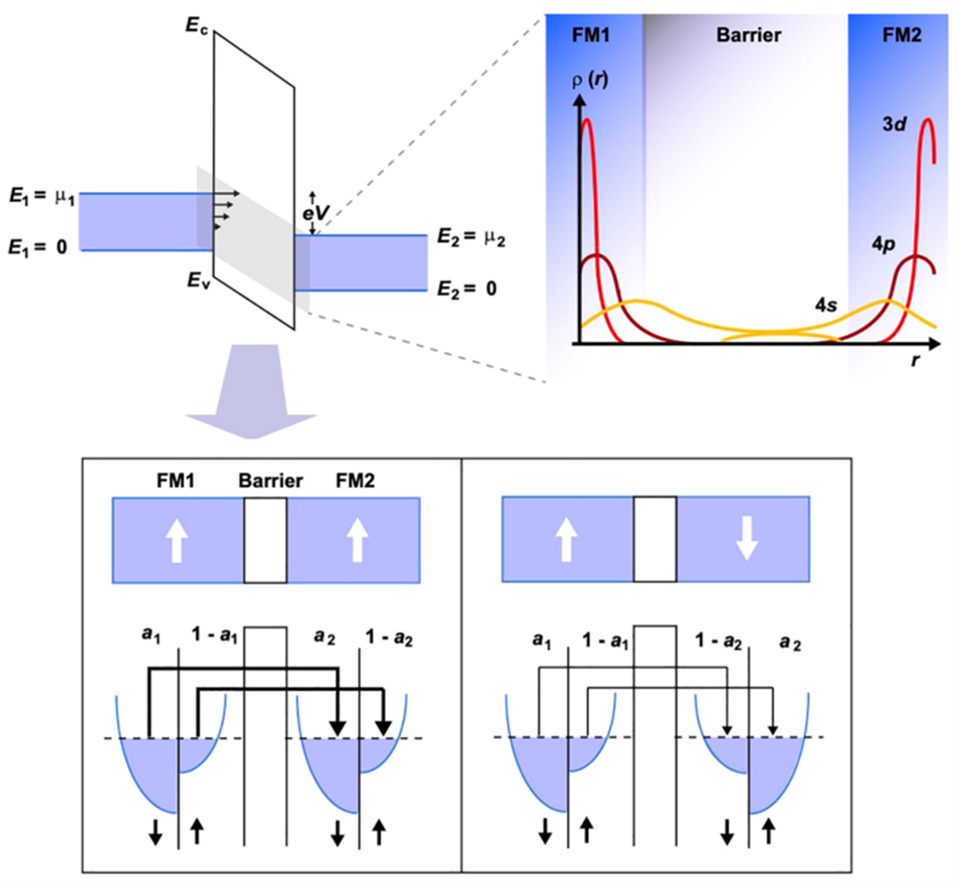
\includegraphics[width=0.6\textwidth]{Figures/Chapter1/图片2.png}
    \bicaption{自旋极化电子隧穿示意图\cite{hirohata2020review}}{Schematic diagram of spin-polarized electron tunnelling\cite{hirohata2020review}}
    \label{图1.2}
\end{figure}
\subsection{自旋霍尔效应(SHE)}
自旋霍尔效应(SHE)是一种相对论性的自旋轨道耦合现象,它可用于在非磁性系统中生成或检测自旋电流。
SHE早在50年前就被预测,理论学家Dyakonov\cite{dyakonov1971current}和Perel\cite{d1971possibility}提出,在相对论性自旋轨道耦合的系统中,非极化电流能够导致横向自旋电流。
在他们的理论中,自旋轨道耦合通过电子在非极化杂质上的Mott散射产生了SHE,这导致具有相反自旋的电子空间分离。
因为自旋的极化轴垂直于横向自旋电流和纵向电流的驱动平面,因此该效应具有霍尔对称性。\par
在提出这一原始理论近30年后,Hirsch\cite{hirsch1999spin}和Zhang\cite{zhang2000spin}引入了实验探测该现象的概念。
Hirsch提出了一种器件,其中自旋电流通过SHE在器件的一个部分产生,并注入到另一个部分,在那里通过逆自旋霍尔效应(iSHE)被检测。
在iSHE中,自旋电流产生一个横向电流,当电荷在样品的边缘积累时,可以通过电学方法检测到。
同时依赖SHE和iSHE来观察此现象的方法在实验上面临着很大的挑战,因此这种方法直到最近才被实现\cite{brune2010evidence}。
然而,SHE有一个逆向对应物的提议在建立该现象的基本物理规律和利用该效应作为非磁性材料中注入和检测自旋电流的工具方面发挥了关键作用。\par
Zhang提出了使用附加的铁磁探针探测由SHE产生的边缘自旋积累的方法。
该方法基于检测铁磁电极上的电化学势与其磁化方向及其下方非磁性体系中积累的自旋的相对取向之间的依赖关系。
这种方法的可行性证明花费了几年的时间。
然而,从更广泛的角度来看,将SHE与在非磁性体系中利用铁磁体注入和检测自旋的领域联系起来的想法,推动了大量重要的自旋霍尔器件的研究。\par
SHE的实验发现源于从不同角度研究SHE的理论工作。
受到有关铁磁体中类似反常霍尔效应的内在本质研究的启发,Murakami等人和Sinova等人预测非磁性体系中电子的自旋相关横向偏转可以直接来自导体的相对论性能带结构,而不涉及Mott散射。
与Hirsch和Zhang提出的利用电学方案检测外在、散射诱导的SHE不同,内在SHE聚焦于半导体,并利用这些材料的光学活性来检测SHE。
Kato等人使用磁光科尔显微镜扫描隧道中的自旋极化,如图\ref{图1.3}所示。
Wunderlich等人使用共面P-N二极管检测自旋霍尔通道相反边缘的圆偏振电致发光。
值得注意的是,Wunderlich等人将观察到的信号归因于内在SHE,而Kato等人将其归因于外在SHE。
\begin{figure}[h]
    \centering
    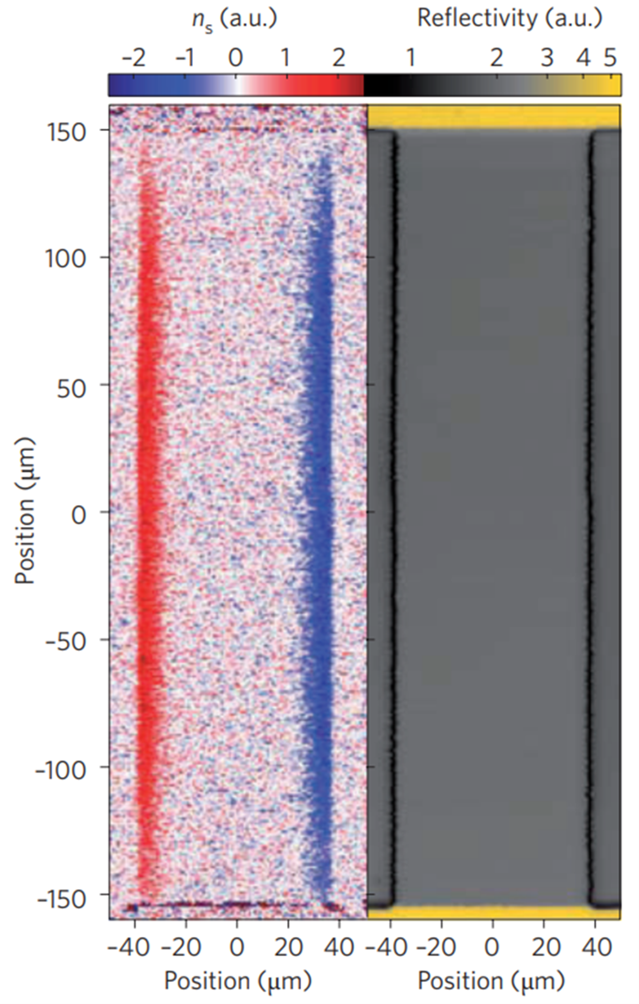
\includegraphics[height=0.31\textheight]{Figures/Chapter1/图片3.png}
    \bicaption{磁光科尔显微镜观察到的SHE}{Observation of SHE by the magneto-optical Kerr microscope}
    \label{图1.3}
\end{figure}
\section{斯格明子研究进展}
磁斯格明子是一种手性自旋结构,它在1989年被预测可以存在于破缺反演对称的磁性材料中。
2009年,M\"uhlbauer等人在低温下(大约\mySI{29}{K})利用中子散射技术首次观测到斯格明子晶格结构存在于手性磁体MnSi中。
随后,在非中心对称的B20化合物以及具有界面Dzyaloshinskii-Moriya相互作用(DMI)的多层结构(铁磁体和重金属的堆叠)中也发现了斯格明子。
由于其非凡的拓扑性质,斯格明子可以被视为局域准粒子并表现出与其拓扑性质相关的静态和动态特性。
在二维体系下,斯格明子的拓扑结构由其拓扑电荷数表征:
\begin{equation}
    Q = \frac{1}{4\pi}\int \bm{m} \cdot \left( \partial_x \bm{m} \times \partial_y \bm{m} \right) \dif x \dif y
    \label{公式1-4}
\end{equation}
式中:$\bm{m}$是单位磁化矢量场。
$Q$表示在整个平面空间内$\bm{m}$绕二维表面的圈数。
最常见的斯格明子包括Bloch型和N\'eel型斯格明子,其拓扑电荷数均为$Q=-1$,如图\ref{图1.4}所示。
\begin{figure}[htb]
    \centering
    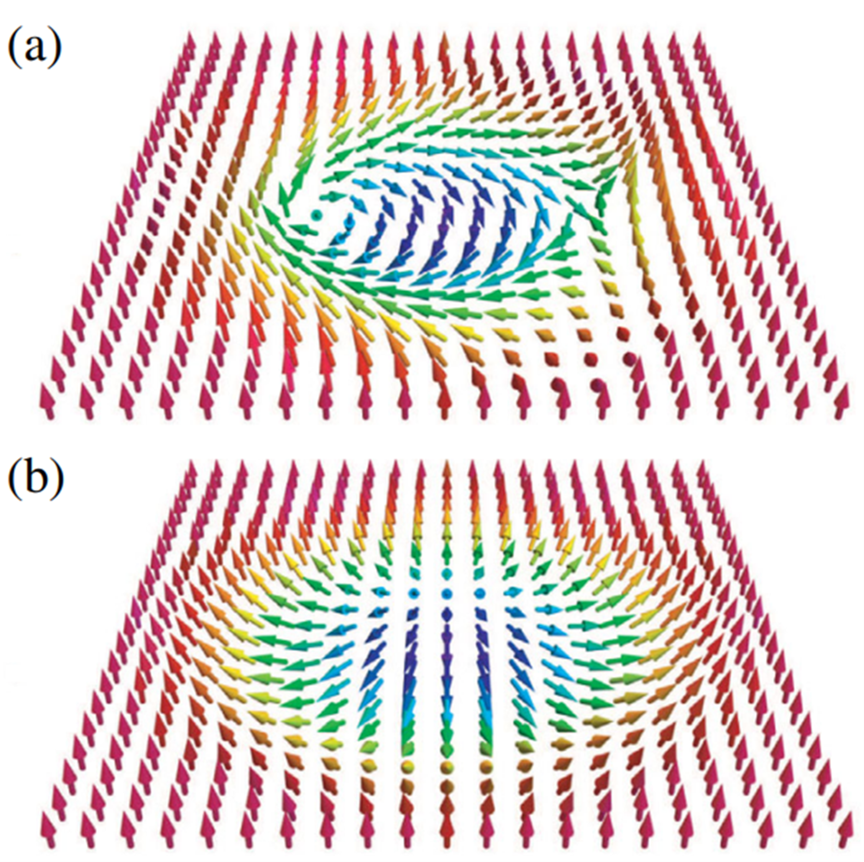
\includegraphics[width=0.5\textwidth ,trim=0cm 0cm 0cm 0.2cm,clip]{Figures/Chapter1/图片4.png}
    \bicaption{不同类型斯格明子的磁化结构}{Magnetization configurations of different types of skyrmion}
    \subcaption*{(a) Bloch型斯格明子;(b) N\'eel型斯格明子}
    \label{图1.4}
\end{figure}\par
自旋极化电流通过对磁矩产生自旋转移力矩(STT)或自旋轨道力矩(SOT)从而推动斯格明子运动,这是斯格明子应用于自旋电子器件重要的驱动力之一。
此外,自旋极化电流也可以用来创建斯格明子。
因此,自旋电流产生和驱动斯格明子在新一代电子器件和信息存储技术方面具有巨大潜力,这体现在它们可以提供更高的存储密度、更快的数据处理速度、更好的稳定性和抗干扰性。\par
2017年,Legrand等人通过在Co多层膜中注入自旋极化电流形成了斯格明子。
如图\ref{图1.5}\hyperlink{子图1.5}{(a)}所示,他们在不同厚度的Co多层膜上注入了1000个持续时间为\mySI{200}{ns}的电流脉冲后形成了多个直径小于\mySI{100}{nm}的斯格明子。在此基础上,他们还研究了电流($J = 2.85\times 10^{11}$\mysi{A/m^2})驱动斯格明子的运动,这些结果有助于设计电流控制的斯格明子器件。
\begin{figure}[htb]
    \hypertarget{子图1.5}{}
    \centering
    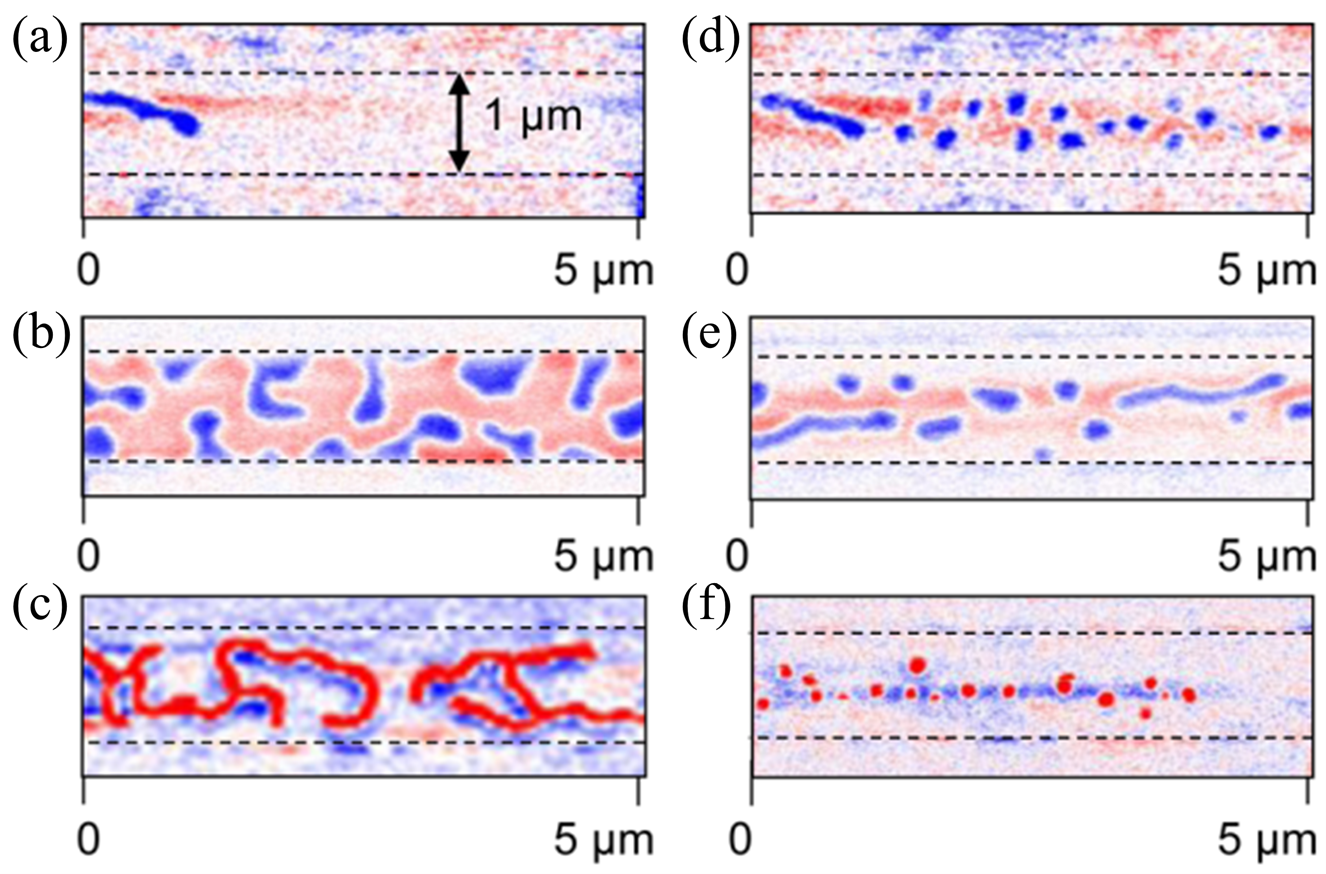
\includegraphics[width=0.8\textwidth]{Figures/Chapter1/图片5.png}
    \bicaption{在具有不同厚度且宽度为\mySI{1}{\micro \meter}的Co多层膜上注入电流前后其磁化结构的变化}{The change in magnetic structure before and after injecting current on Co multilayers with different thicknesses and a width of \SI{1}{\micro \meter}}
    \subcaption*{(a)-(c) 注入电流前且Co的厚度分别为\mySI{0.6}{nm},\mySI{0.8}{nm},\mySI{1.0}{nm}时的磁化结构;
    (d)-(f) 注入电流后且Co的厚度分别为\mySI{0.6}{nm},\mySI{0.8}{nm},\mySI{1.0}{nm}时的磁化结构}
    \label{图1.5}
\end{figure}
\subsection{斯格明子赛道存储器}
斯格明子的拓扑结构稳定、纳米级尺寸和驱动电流密度低等特点使它有望成为下一代自旋电子器件的信息载体,而斯格明子最有潜力的应用之一是赛道存储器。
2013年,Fert等人提出可以使用斯格明子来建立磁赛道存储器,它类似基于磁畴壁的磁赛道存储器。
在基于斯格明子的磁赛道存储器中,信息可以通过斯格明子的存在和不存在来编码,例如让斯格明子的存在表示数据位“1”,缺失表示数据位“0”,如图\ref{图1.6}所示。
2015年,Tomasello等人展示了通过在铁磁层或重金属基底中产生自旋霍尔效应引起的自旋电流来操纵Bloch型和N\'eel型斯格明子的技术优势和局限性。
他们发现,由自旋霍尔效应引起的自旋力矩驱动N\'eel型斯格明子是实现下一代斯格明子赛道存储器最有前途的方法。
2017年,Yu等人在实验上实现了一种室温下基于斯格明子运动的存储器件,这为建立完全功能的斯格明子赛道存储器提供了基础。\par
然而,这种方法在读取赛道中的长序列数据位时并不稳定,尤其是考虑到热扰动的影响。
例如,对于一个由“0”位(即缺失斯格明子)组成的数据序列,实际上很难确定纳米轨道中传输了多少个“0”数据位,因为两个斯格明子之间的间距可能是变化的。
此外,时钟同步是一个难以解决的问题,因为数据位“0”的位置是不可预测的。
2016年Wang等人提出了一种新型赛道存储器模型以解决上述问题。
通过电压调控,他们将“0”和“1”两种数据位均用存在斯格明子表示,并将它们同步移动,如图\ref{图1.7}所示。
利用电压控制的Y形结构赛道,可以将斯格明子驱动到L型或R型纳米轨道中,具体取决于输入的数据位,如图\ref{图1.7}\hyperlink{子图1.7}{(b)}所示。
例如,如果输入数据位为“0”,则开启L支路并关闭R支路使斯格明子移动到L型纳米轨道。
如果输入的数据位是“1”,斯格明子将移动到R型纳米轨道中。
\begin{figure}[H]
    \centering
    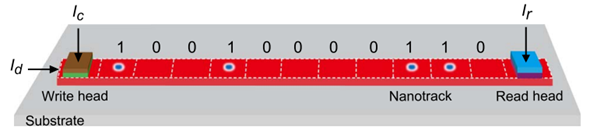
\includegraphics[width=\textwidth]{Figures/Chapter1/图片6.png}
    \bicaption{斯格明子用于信息编码的赛道模型}{Skyrmion racetrack model for information encoding}
    \label{图1.6}
\end{figure}\par
需要注意的是,当斯格明子被驱动到其中一条纳米轨道时,与之对应的铁磁态(无斯格明子状态)也会同时被驱动到另一条纳米轨道,因为两条纳米轨道的驱动电流是同时打开的。
这样就可以形成互补型的数据表示,并且可以通过区分斯格明子的位置(在L型纳米轨道或R型纳米轨道中)来检测数据位。
互补型斯格明子赛道存储器的设计大大提高了斯格明子检测的稳定性。
\begin{figure}[h]
    \hypertarget{子图1.7}
    \centering
    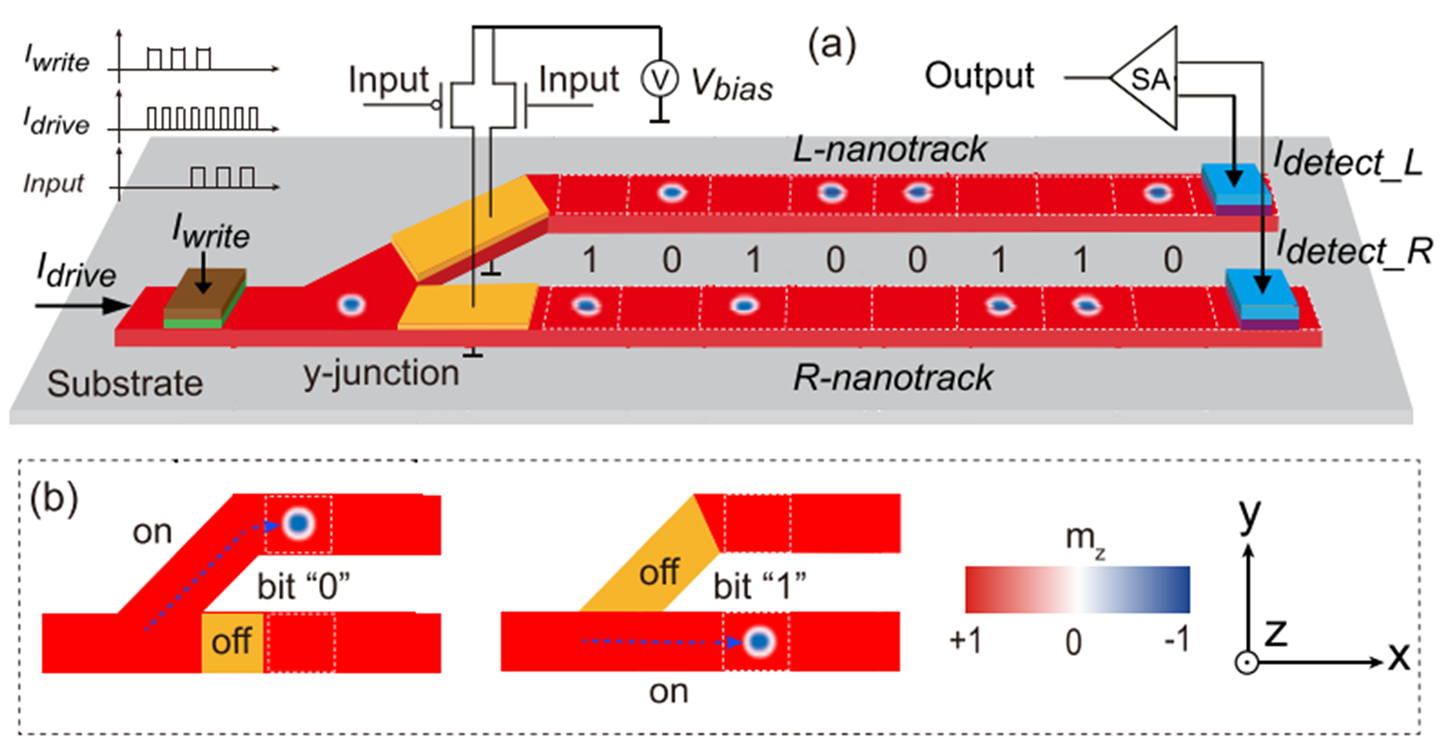
\includegraphics[width=\textwidth]{Figures/Chapter1/图片7.png}
    \bicaption{互补型斯格明子赛道存储器}{Complementary skyrmion racetrack memory}
    \subcaption*{(a) 存储器模型示意图;(b) 电压控制的Y型结构的数据表示和编码}
    \label{图1.7}
\end{figure}
\subsection{斯格明子霍尔效应}
斯格明子作为一种具有类似粒子特性的磁化结构,其拓扑电荷不为零,这使它在运动时方向会发生偏转,就像带电粒子在磁场中的运动,这被称为斯格明子霍尔效应(SkHE),这种使斯格明子运动时方向发生偏转的力被称为马格努斯力。
当斯格明子应用于赛道存储器时,它可能会因为马格努斯力的存在而运动到赛道边缘并湮灭,但是当斯格明子应用于逻辑器件时,马格努斯力的存在会使斯格明子的运动轨迹偏转从而实现某种逻辑运算。
因此研究SkHE对于斯格明子的应用是十分必要的。\par
2017年,Jiang等人研究电流驱动斯格明子时,使用磁光科尔(MOKE)显微镜在室温下CoFeB中直接观察到了SkHE,如图\ref{图1.8}所示。
他们通过施加不同方向的电流来驱动具有不同拓扑电荷($Q = +1$和$Q = -1$)的斯格明子,揭示了带电粒子的传统霍尔效应和斯格明子的SkHE之间的强相关性。
此外,他们发现当斯格明子在靠近赛道边缘运动时,斯格明子会同时受到驱动力、马格努斯力和边缘排斥力的影响,这也会影响它的运动轨迹发生变化。
\begin{figure}[h]
    \centering
    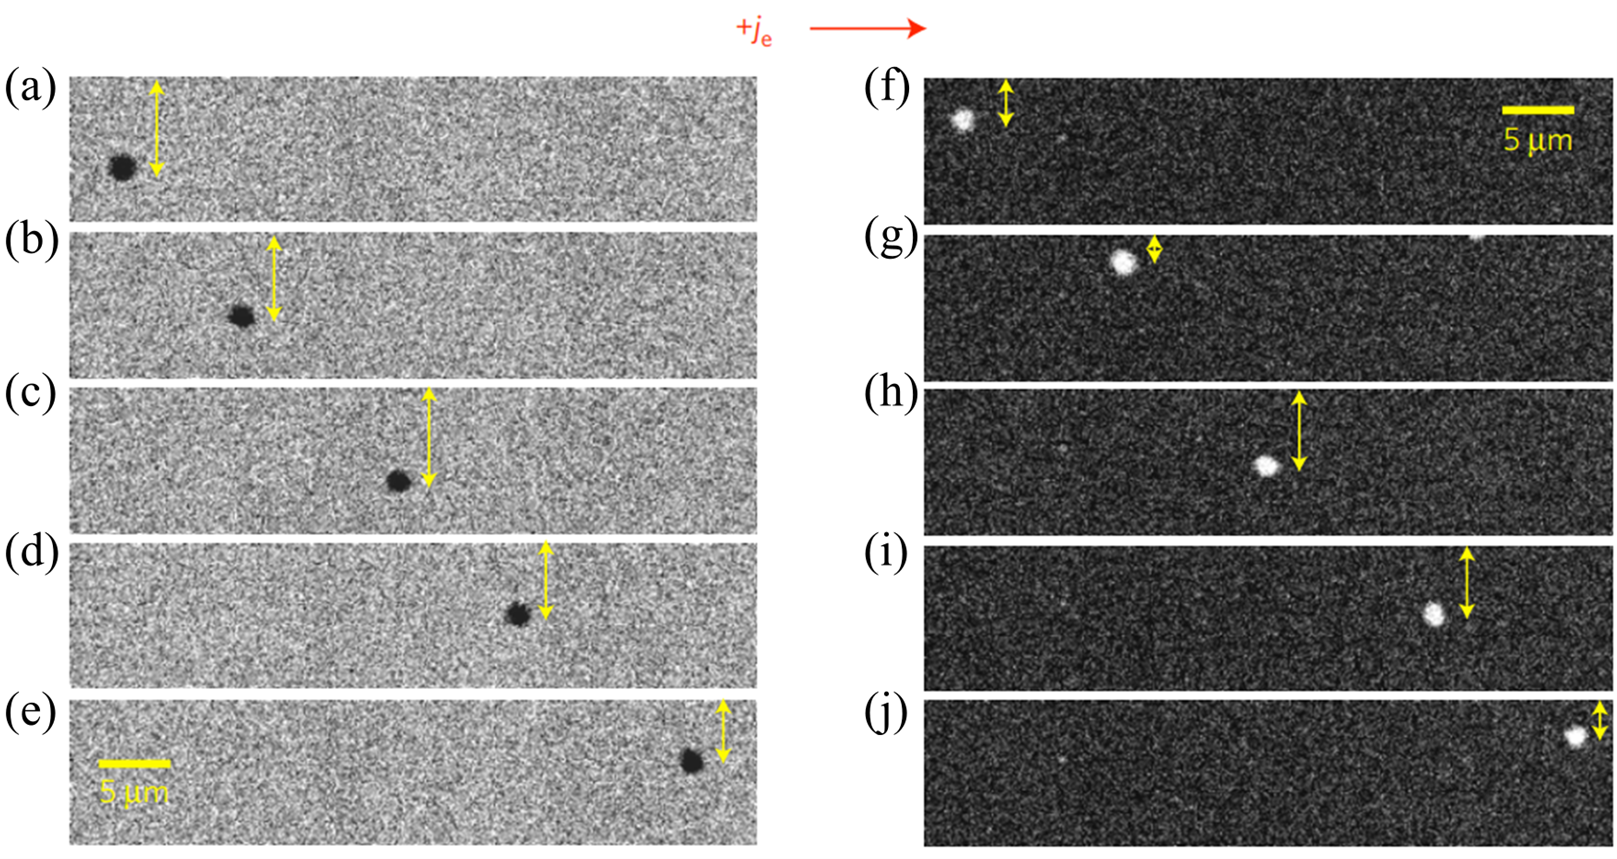
\includegraphics[width=\textwidth]{Figures/Chapter1/图片8.png}
    \bicaption{脉冲电流驱动斯格明子运动的MOKE显微镜图像}{MOKE microscopy images of pulse current-driven skyrmion motion}
    \subcaption*{(a)-(e) $Q = -1$ 的斯格明子的运动轨迹;
    (f)-(j) $Q = +1$的斯格明子的运动轨迹}
    \label{图1.8}
\end{figure}\par
2019年,Juge等人研究了在室温下Pt/Co/MgO薄膜上电流驱动斯格明子的动力学。
他们使用扫描电子显微镜(SEM)观测到了斯格明子,计算得到在电流驱动下斯格明子的最快速度可达到\mySI{100}{m/s},并发现斯格明子的运动过程伴随着相应的SkHE,如图\ref{图1.9}所示。
此外,他们通过微磁模拟研究了SOT和材料缺陷对于斯格明子的运动速度以及SkHE的不同影响机制,结果表明材料缺陷(钉扎)对SkHE起主导性作用。
这些结果对基于斯格明子的应用具有重要作用。
\begin{figure}[htb]
    \centering
    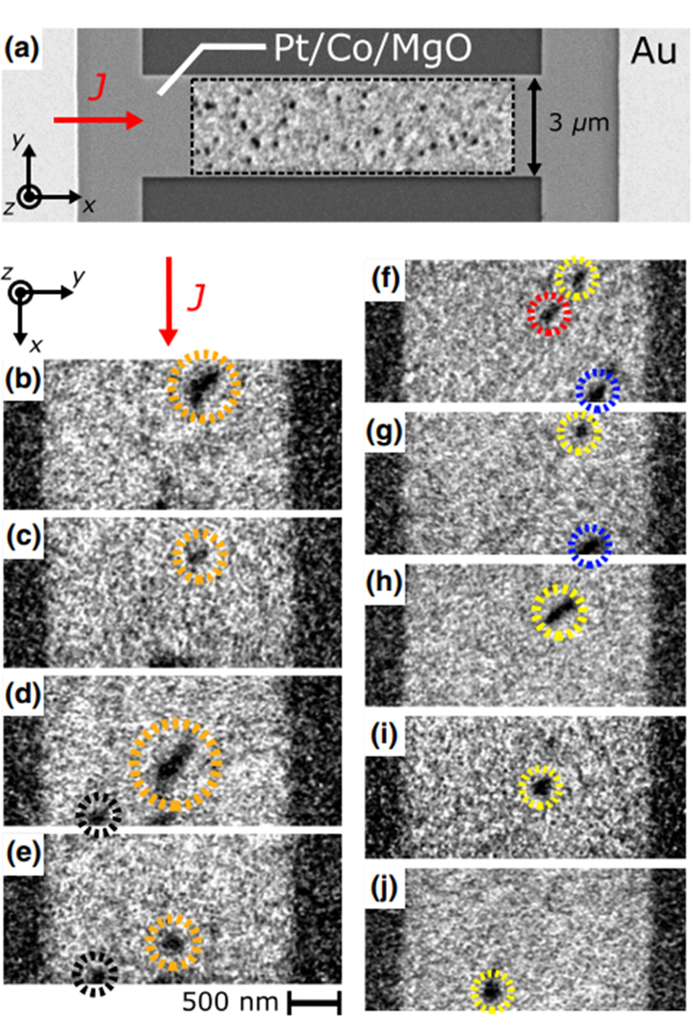
\includegraphics[width=0.45\textwidth]{Figures/Chapter1/图片9.png}
    \bicaption{电流驱动斯格明子的模型及运动过程}{Model and motion process of current-driven skyrmion}
    \subcaption*{(a) 模型的SEM图像,包括一个\mySI{3}{\micro\meter}宽的Pt/Co/MgO赛道和与之接触的Ti/Au垫片用来注入电流;(b) 电流驱动斯格明子的运动过程}
    \label{图1.9}
\end{figure}
\subsection{斯格明子二极管}
二极管是一种具有使电流单向导通特性的半导体元件,已被广泛应用于计算、通信、传感等领域,它极大的促进了当代科学的发展。
受到电子二极管单向导通性能的启发,研究人员将目光投向其它可能实现单向导通性的领域,如微流体、光、热、磁等。
其中磁斯格明子具有拓扑结构稳定、运动速度快以及尺寸小等优势,这使它能够作为信息载体并应用于二极管。\par
2020年Zhao等人设计了一个基于斯格明子的二极管模型,并通过微磁模拟证明了斯格明子在该模型下能够实现单向导通,如图\ref{图1.10}所示。
他们通过压控磁各向异性(VCMA)技术提高赛道边缘的垂直磁各向异性(PMA),这不仅能够通过减小SkHE来防止斯格明子湮灭,还能够有效提高斯格明子的运动速度。
此外,调节驱动电流大小以及VCMA门宽度等参数可以控制斯格明子正向的导通和反向的钉扎。
这对于斯格明子二极管的设计提供了新的思路。
\begin{figure}[htb]
    \centering
    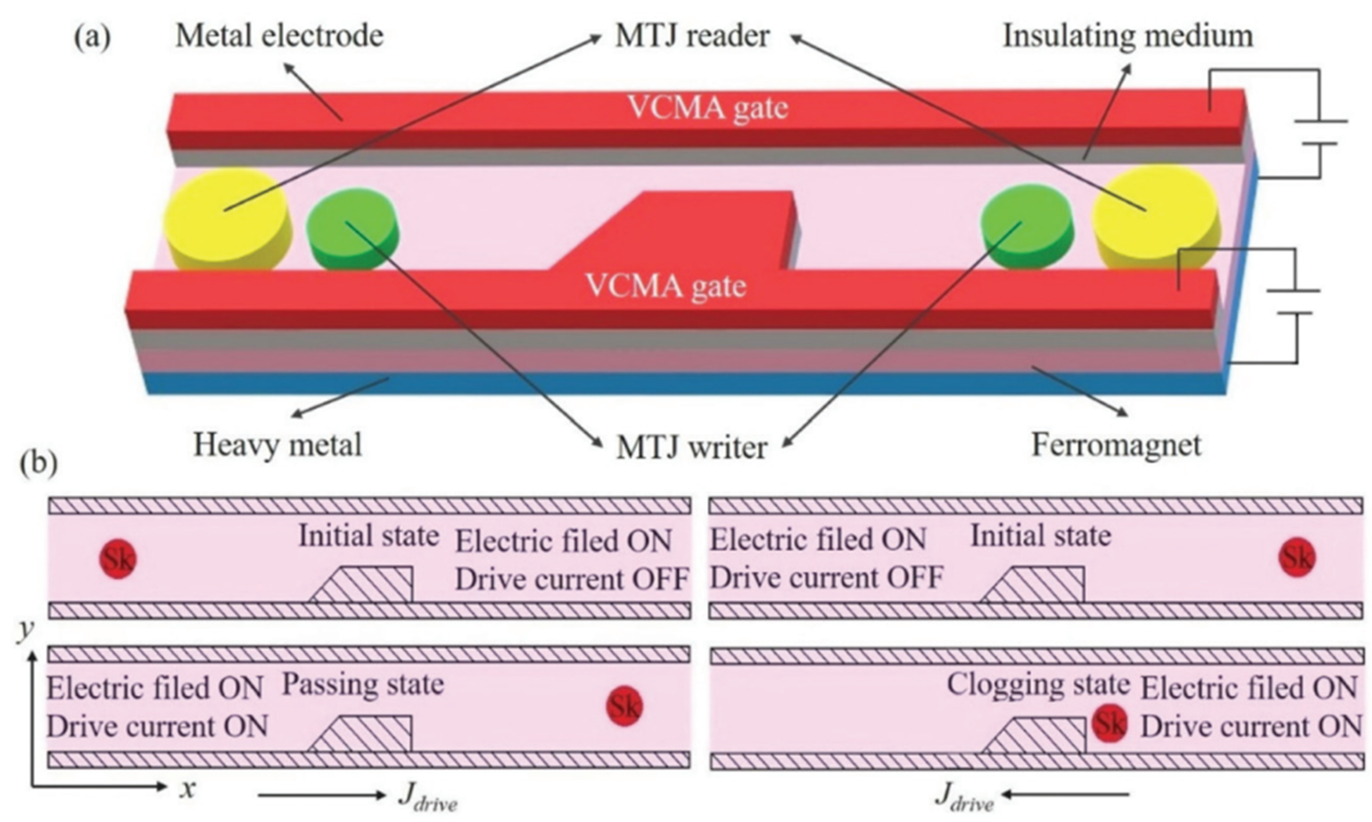
\includegraphics[width=0.8\textwidth]{Figures/Chapter1/图片10.png}
    \bicaption{基于斯格明子二极管的模型及其单向导通性}{Schematic of the skyrmion-based diode and the one-way motion of the skyrmion}
    \subcaption*{(a) 基于斯格明子的二极管模型;(b) 斯格明子正向导通和反向钉扎}
    \label{图1.10}
\end{figure}\par
2022年,Feng等人利用SkHE设计了斯格明子二极管。
当斯格明子沿赛道从左向右运动时,它受到驱动力、马格努斯力和赛道上边缘的排斥力,这使它能够到达赛道右端。
当斯格明子从右向左运动时,它受到的合力使斯格明子向赛道下边界运动并湮灭,如图\ref{图1.11}所示。
此外,他们还研究了斯格明子在这种非对称赛道中运动的动力学以及热扰动下斯格明子的稳定性,这对于设计斯格明子二极管具有重要作用。
\begin{figure}[H]
    \centering
    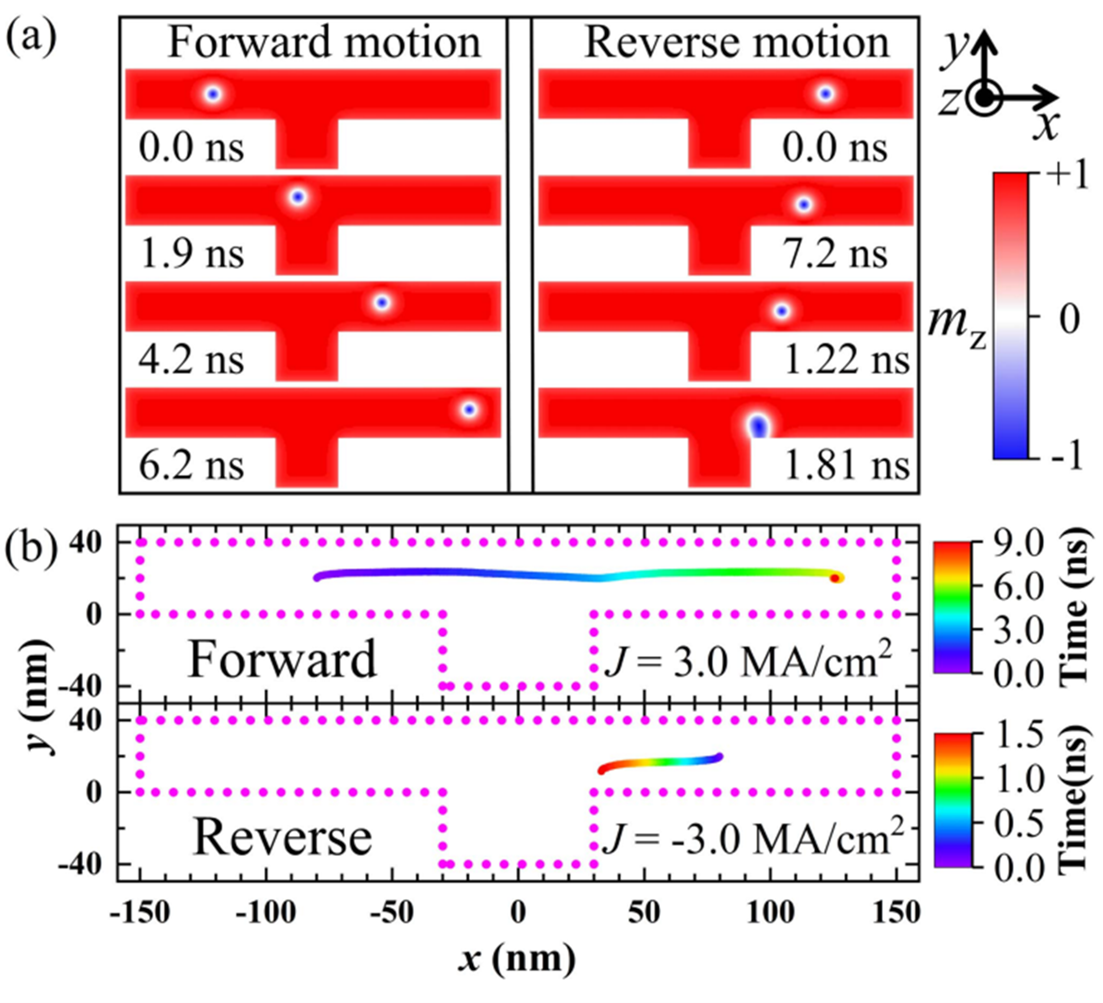
\includegraphics[width=0.7\textwidth]{Figures/Chapter1/图片11.png}
    \bicaption{斯格明子在非对称结构赛道中的运动}{Skyrmion motions in the asymmetric structure racetrack}
    \subcaption*{(a) 斯格明子的运动过程;(b) 斯格明子的运动轨迹}
    \label{图1.11}
\end{figure}
\section{斯格明子袋研究进展}
斯格明子袋是一种稳定的、具有高拓扑度和类似斯格明子的磁化结构,它由一个大的斯格明子嵌套任意数量的内部反斯格明子组成,如图\ref{图1.12}所示。
在磁性薄膜中,可以通过总的拓扑电荷数$Q$来描述斯格明子袋,见公式(\ref{公式1-4})。
$Q = -1$表示一个斯格明子;$Q = +1$表示斯格明子袋内的一个反斯格明子。
这里,可以用符号S(N)来表示由一个外部斯格明子和任意数量的内部反斯格明子组成的斯格明子袋,其中N是内部反斯格明子的数量,斯格明子袋的总拓扑数为$Q = N-1$。
换句话说,S(0)表示一个斯格明子,S(N) (N > 0)代表有N个内部反斯格明子的斯格明子袋。
\begin{figure}[htb]
    \centering
    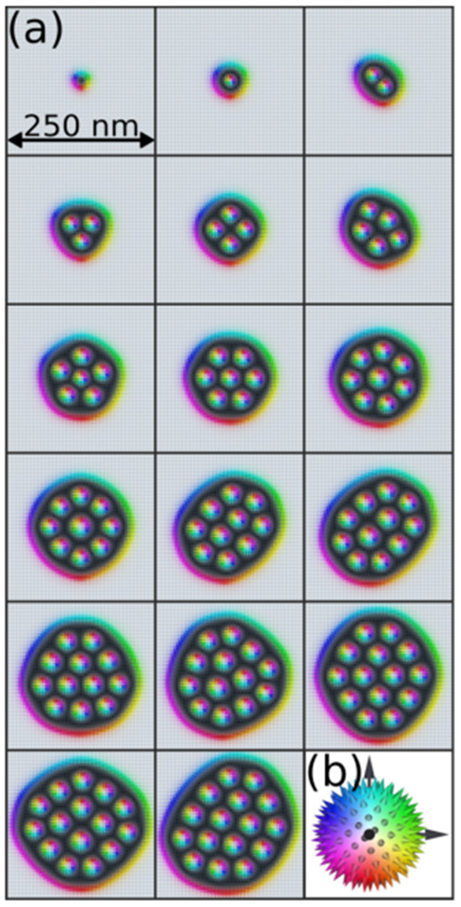
\includegraphics[width=0.3\textwidth]{Figures/Chapter1/图片12.png}
    \bicaption{斯格明子袋的磁化结构}{Magnetic configurations of skyrmion bags}
    \subcaption*{(a) 使用MuMax3模拟的S(N) (N = 0 - 16);(b) 使用Runge色球表示S2上的方向}
    \label{图1.12}
\end{figure}
\subsection{斯格明子袋在实验中的发现}
当斯格明子应用于赛道存储器时,一个斯格明子只能代表一个二进制位比特,而且斯格明子之间的排斥力决定了存储密度的上限。
此外,实际的磁性材料是具有缺陷和杂质的,这会影响斯格明子移动并可能导致信息编码发生错误。在这样的背景下,将斯格明子替换为斯格明子袋将可能解决上述问题。\par
2019年,Foster和Kind等人通过实验证明了斯格明子袋可以稳定存在于液晶中,并且通过微磁模拟的方法研究了它在磁性材料中的性质。
研究表明,在FeGe薄膜中斯格明子袋在\mySI{1}{MA/cm^2}的电流驱动下达到的速度约为\mySI{1}{m/s}。
他们通过对具有不同磁化结构的斯格明子袋赋予不同的二进制位信息,成功表达出了单词“SKYRME”,如图\ref{图1.13}所示。
此外,斯格明子袋之间的排斥力随着距离的减小而显著增大,这也类似于斯格明子之间的相互作用,如图\ref{图1.14}所示。
这表明斯格明子袋在运动过程中不会发生碰撞而湮灭。
\begin{figure}[H]
    \centering
    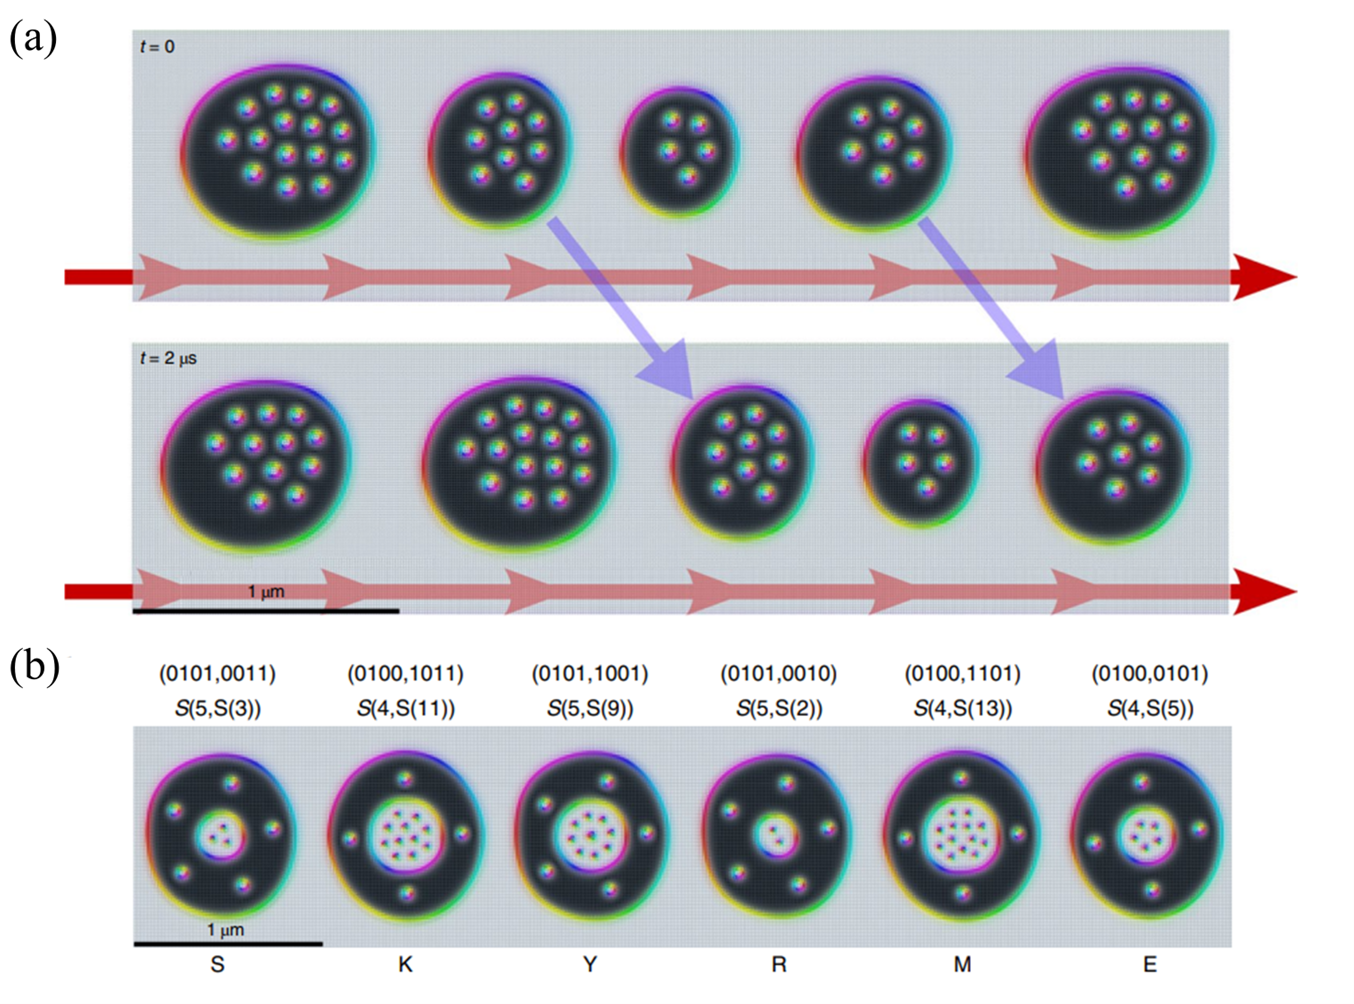
\includegraphics[width=0.8\textwidth]{Figures/Chapter1/图片13.png}
    \bicaption{电流驱动斯格明子袋运动和不同拓扑度斯格明子袋的信息编码}{Current-induced motions and data encoding of skyrmion bag}
    \subcaption*{(a) 电流驱动斯格明子袋运动的不同阶段;
    (b) 使用ACSII二进制编码的单词“SKYRME”,其中外面的斯格明子袋表示前四位比特,内部的斯格明子袋表示后四位比特,每个完整的斯格明子袋代表一个字母}
    \label{图1.13}
\end{figure}
\begin{figure}[H]
    \centering
    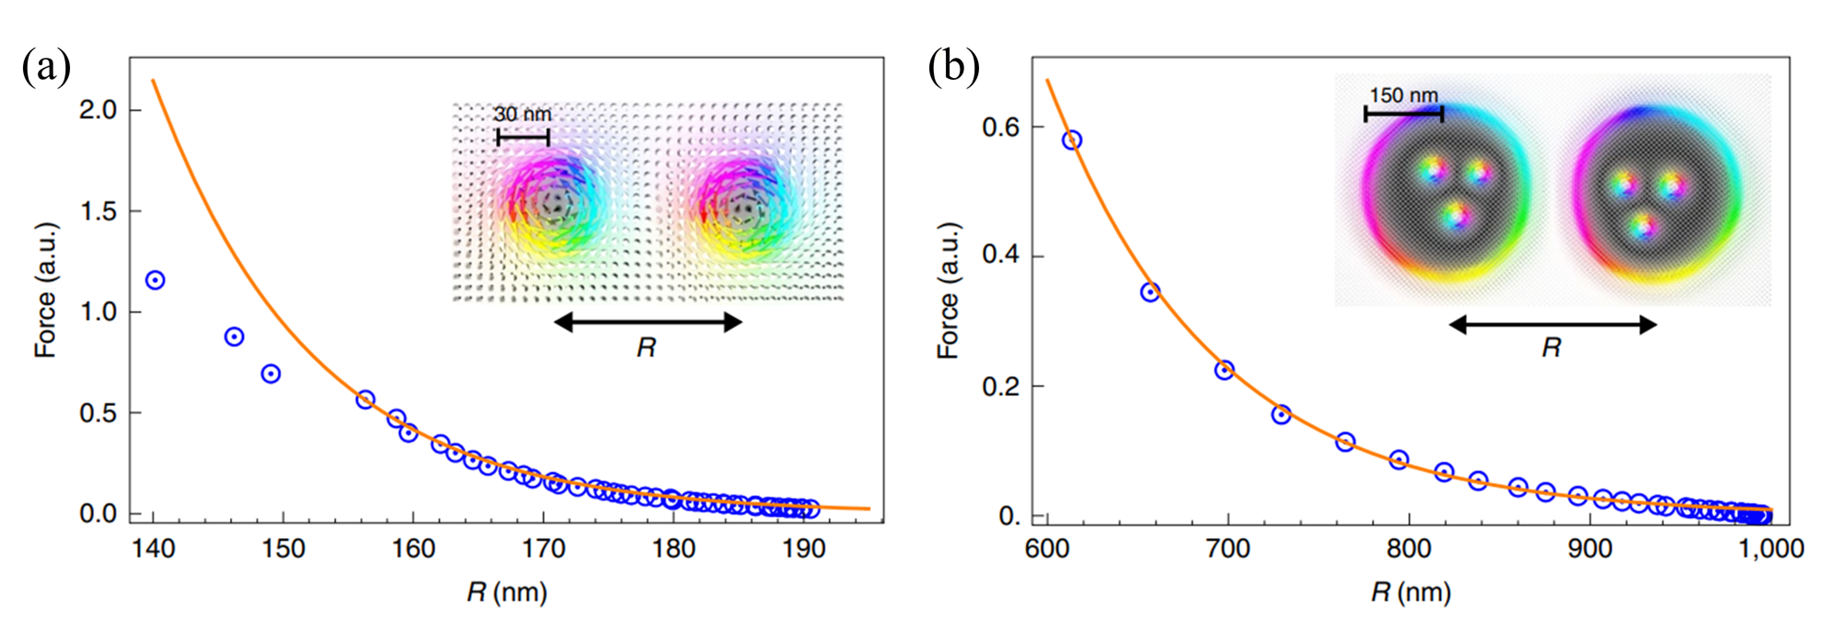
\includegraphics[width=\textwidth]{Figures/Chapter1/图片14.png}
    \bicaption{斯格明子和斯格明子袋之间的排斥力随它们间距的变化}{The repulsive force as a function of distance of skyrmions and skyrmion bags}
    \subcaption*{(a) 斯格明子之间的排斥力随间距的变化;(b) 斯格明子袋之间的排斥力随间距的变化}
    \label{图1.14}
\end{figure}\par
2021年,Tang等人使用洛伦兹透射电子显微镜(LTEM)在厚度为\mySI{150}{nm}的FeGe片中观测到了三维斯格明子袋,并研究了电流脉冲对它的影响。
图\ref{图1.15}显示了斯格明子束(skyrmion bundle)的磁化结构,其内部截面为斯格明子袋。
他们从实验上证明了斯格明子束是一种稳定并具有高拓扑度的磁化结构,它在电流驱动下也具有斯格明子霍尔效应,并且斯格明子霍尔角随斯格明子袋的拓扑电荷变化而变化。
这对于在二维手性磁体中实现斯格明子袋并进一步应用于高密度赛道存储器具有重要意义。
\begin{figure}[htb]
    \centering
    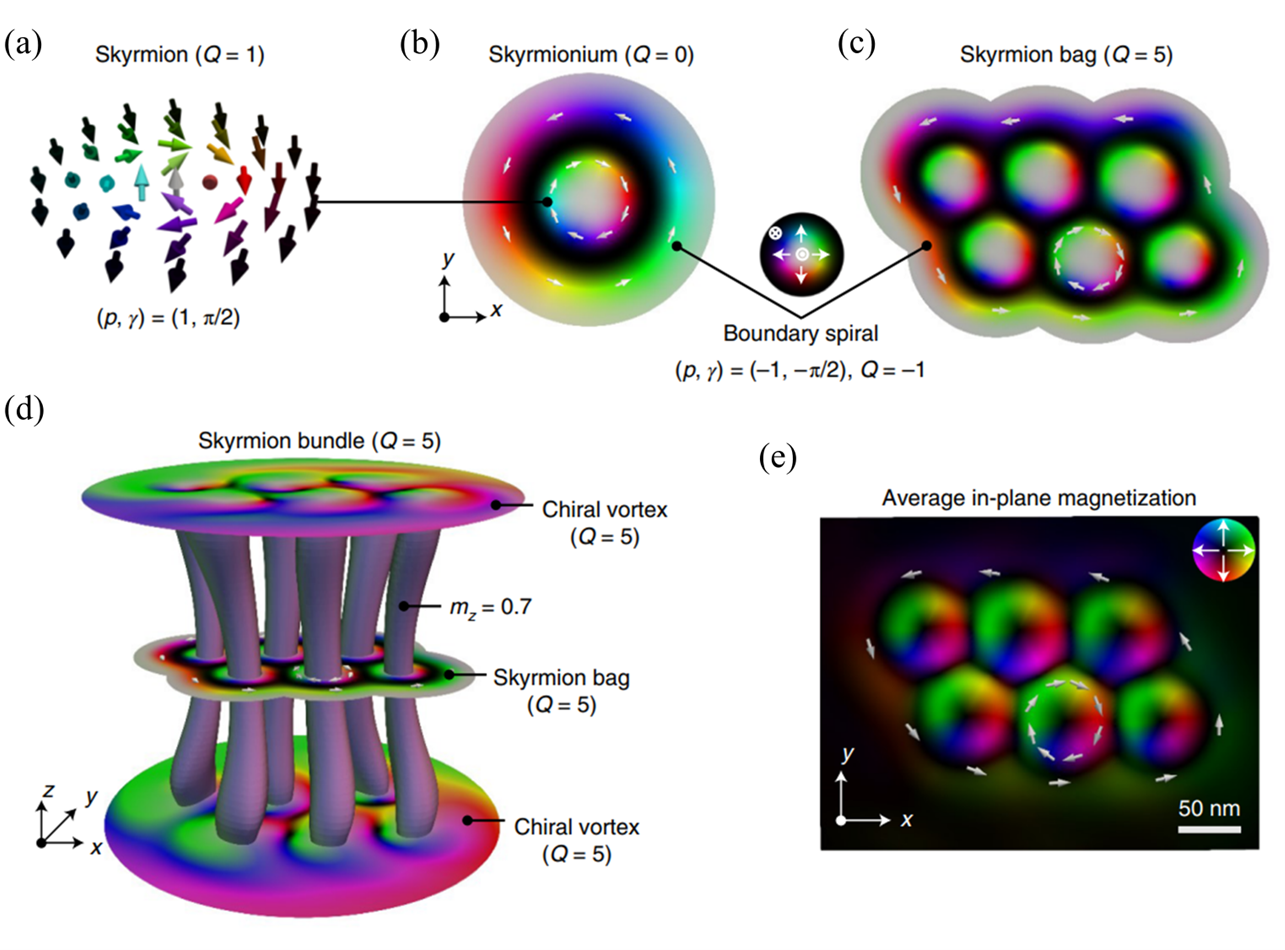
\includegraphics[width=0.65\textwidth]{Figures/Chapter1/图片15.png}
    \bicaption{磁斯格明子束的示意图}{Schematics of a magnetic skyrmion bundle}
    \subcaption*{(a) 拓扑电荷$Q=1$的斯格明子;
    (b) $Q=0$的嵌套斯格明子(skyrmionium);
    (c) $Q=5$的斯格明子袋;
    (d) 在厚度为\mySI{150}{nm}的FeGe片中的$Q=5$的斯格明子束;
    (e) 斯格明子束的面内磁化结构}
    \label{图1.15}
\end{figure}
\subsection{斯格明子袋在电流驱动下的特性}
斯格明子袋能够像斯格明子一样在各种驱动方式下运动,如自旋极化电流和PMA梯度。
由于斯格明子在电流驱动下能够表现出速度快和结构稳定等优势,因此研究人员更愿意将注意力放到电流驱动斯格明子的动力学。
同理,电流驱动斯格明子袋的研究也正在吸引越来越多的研究人员。
斯格明子袋在电流驱动下表现出的动力学特性(如速度和霍尔角等)与其自身的拓扑电荷数相关,这对于具有不同拓扑数的斯格明子袋应用于赛道存储器是十分有意义的。\par
2020年,Wang等人利用微磁模拟研究了斯格明子袋在SOT的驱动下的动力学。
他们发现在具有周期性边界条件下的Co/Pt多层膜中用相同大小的电流驱动斯格明子袋时,斯格明子袋的速度随着其拓扑数的增加而逐渐减小,但斯格明子霍尔角随着它的拓扑数增加而增大;
在无周期性边界条件的Co/Pt纳米条带上驱动斯格明子袋时,斯格明子袋的速度与其拓扑数基本无关,如图\ref{图1.16}所示。
此外,他们证明了斯格明子袋在纳米条带上通过缺陷时仍然能表现出良好的拓扑保护性,如图\ref{图1.17}所示。这使斯格明子袋在应用于新一代自旋电子器件时更具优势。
\begin{figure}[htb]
    \centering
    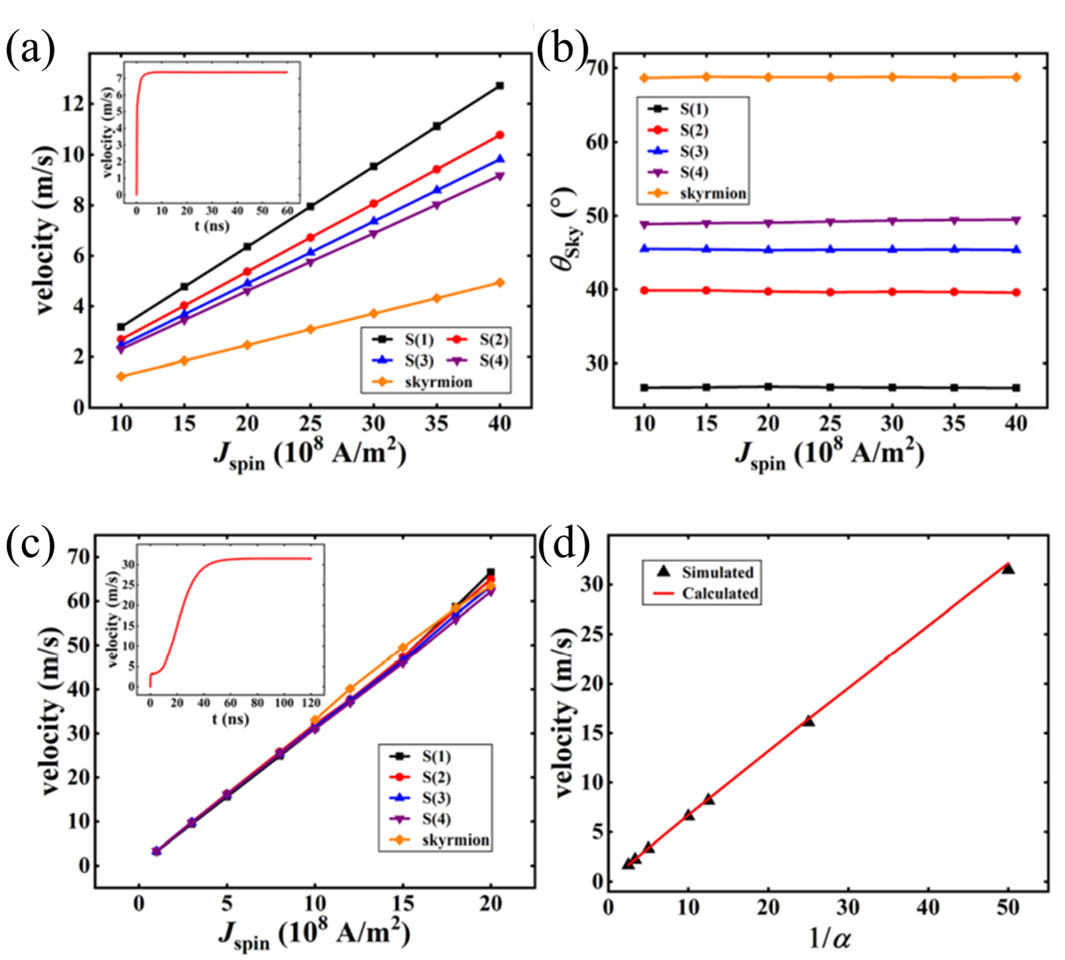
\includegraphics[width=0.6\textwidth]{Figures/Chapter1/图片16.png}
    \bicaption{斯格明子袋在磁性薄膜和纳米条带中的运动}{The motion of the skyrmion bag in the ferromagnetic film and nanostrip}
    \subcaption*{(a)和(b) 磁性薄膜中的斯格明子袋S(N) (N = 1 - 4)和斯格明子在不同电流的驱动下它们的速度和斯格明子霍尔角的变化;
    (c)和(d) 纳米条带中的斯格明子袋S(N) (N = 1 - 4)和斯格明子在不同电流和阻尼系数的条件下它们的速度的变化}
    \label{图1.16}
\end{figure}
\begin{figure}[H]
    \centering
    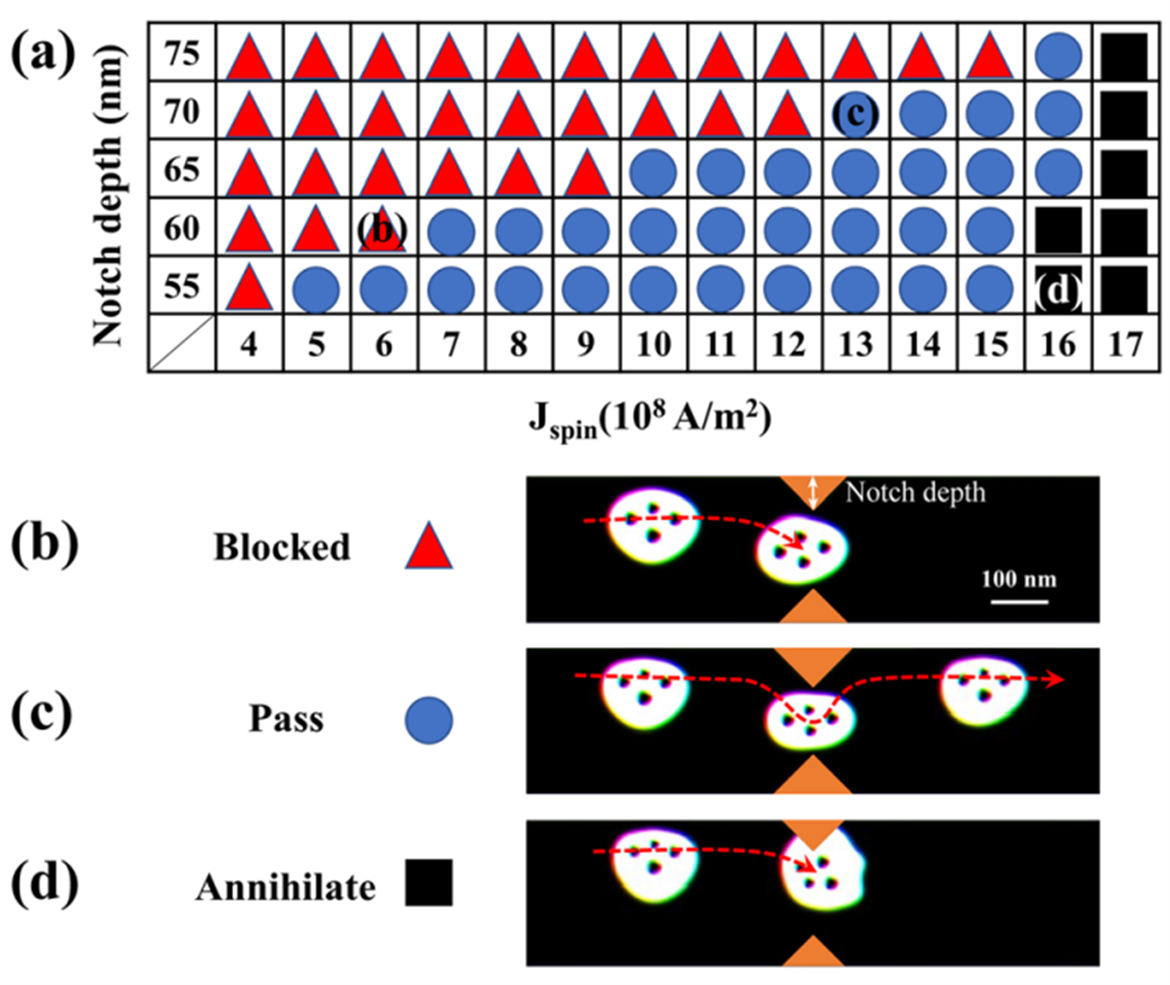
\includegraphics[width=0.6\textwidth]{Figures/Chapter1/图片17.png}
    \bicaption{斯格明子袋通过缺陷时的钉扎状态和过程}{The pining state and process of skyrmion bag passing through a defect}
    \label{图1.17}
\end{figure}\par
2021年,Kind等人研究了平面内电流(CIP)和平面外电流(CPP)驱动具有不同拓扑度的斯格明子袋的动力学。
他们用Thiele方程和微磁模拟研究了在这两种方式的驱动下,磁性薄膜中的斯格明子袋 S(N) (N = 0 - 16)的运动速度和斯格明子霍尔角随其拓扑数的变化。
结果显示,在CIP和CPP驱动下,当S(N)的拓扑度较低时,例如N = 0 - 4,斯格明子霍尔角会发生明显变化;
当S(N)的拓扑度较高时,斯格明子霍尔角几乎不变,并且当N趋于无穷大时,斯格明子霍尔角存在一个极限值。
此外,在相同电流密度下,CPP驱动的S(N)具有更高的速度,但相应的偏转角也更大。
\section{研究内容}
斯格明子是一种特殊的自旋磁化结构并且具有类似粒子的特性。
由于它具有拓扑稳定性好、驱动电流密度低以及尺寸小等优点,斯格明子在自旋电子学和磁学领域被广泛研究。
目前对于斯格明子应用于二极管的研究仍停留在利用赛道结构的非对称性实现斯格明子的单向导通,并未解释斯格明子在运动过程中的速度变化以及相关的动力学行为,更没有得出斯格明子二极管的“伏安特性”曲线。
另一方面,斯格明子袋作为一种嵌套式斯格明子结构,它具有的任意拓扑电荷数使它可以作为高密度赛道存储器的信息载体。
已有研究表明斯格明子袋可以编码为不同的信息,但尚不知如何将斯格明子袋应用于赛道存储器才能实现高密度存储。
本论文通过微磁学模拟的方法,研究在合成反铁磁赛道上电流驱动不同拓扑度的斯格明子通过电压门的动力学。
研究内容包括:
\begin{enumerate}[label=(\arabic*), leftmargin=4ex, labelsep=1.4ex, itemsep=0pt, topsep=1ex,partopsep=1ex,parsep=0pt]
    \item 研究斯格明子从赛道两端开始运动并通过电压门时速度的变化,以及电压门产生的PMA梯度和驱动电流密度对斯格明子运动速度的影响,得到斯格明子的最低速度和驱动电流密度的关系曲线。
    \item 从静态上探讨不同大小的PMA对斯格明子尺寸的影响,以及从动态上研究PMA梯度对运动的斯格明子阻力的大小。
    \item 探讨材料参数(如PMA常数$K_u$、DMI常数$D$、海森堡交换常数$A$)对Co/Pt薄膜磁化结构的影响, 确认最适合斯格明子袋存在的参数范围。
    \item 研究初始态为S(4)的斯格明子袋在电流驱动下通过电压门控制的PMA梯度区域时发生的不同拓扑结构转变,并分析拓扑结构发生转变的原因。
    \item 研究不同初始态的斯格明子袋通过电压门后发生的拓扑转变,并尝试通过在一个赛道上设置多个电压门实现从S(4)到S(1)的连续拓扑转变。
\end{enumerate}
\section{研究目的及意义}
斯格明子是一种具有拓扑保护的纳米自旋结构,它具有尺寸小、拓扑结构稳定和低驱动电流密度等优点。
这些特性使得斯格明子可以作为赛道存储器、逻辑器件和纳米振荡器中的信息载体。
目前关于斯格明子的形成、稳定和运动等研究已不计其数,这些基础研究对于实现斯格明子的应用奠定了基础。\par
一方面,当斯格明子应用于二极管时,利用赛道结构或者能量的不对称性可以实现斯格明子的单向导通。
但是斯格明子在运动过程中的速度变化以及相关的动力学行为尚未有具体解释。
更重要的是,已有的关于斯格明子二极管的研究没有给出类似电子二极管的 “伏安特性”,这表明斯格明子二极管的研究结果仍不完整。
本论文研究了自旋电流驱动斯格明子在带有VCMA的合成反铁磁赛道上的动力学。
通过分析斯格明子正向和负向通过不同电压门时其最小速度与驱动电流密度和PMA梯度的关系,得到了斯格明子二极管的驱动电流密度—最小速度特性曲线,这类似于电子二极管的伏安特性曲线。
这些工作完善了斯格明子二极管的理论研究。\par
另一方面,当斯格明子应用于赛道存储器时,一个斯格明子只能代表一个二进制位信息,并且斯格明子之间的排斥力使它们保持相对较长的距离,这不利于高密度信息存储。
斯格明子袋是具有任意拓扑电荷数的嵌套式斯格明子结构,它可以很好地解决这个问题。
已有研究表明斯格明子袋可以作为不同的编码信息,但是将斯格明子袋应用于赛道存储器的基本理论以及设计思路还没有出现。
本论文提出了一种基于斯格明子袋的高密度赛道存储器,它通过在合成反铁磁赛道上施加自旋极化电流驱动斯格明子袋通过电压门并发生相应的拓扑结构转变来实现。
此外,分析了斯格明子袋发生拓扑转变的根本原因,它与内部反斯格明子之间的相互作用力的变化有关。
在此理论基础上,进一步通过在一个赛道上设置三个电压门实现了斯格明子袋从S(4)到S(1)的连续拓扑转变。
这些结果为实现基于斯格明子袋的高密度赛道存储器提供了理论基础和设计思路。
\newpage